\documentclass{article}
\usepackage[utf8]{inputenc}
\usepackage{array,multirow}
\usepackage{mathabx}
\usepackage{parskip}
\usepackage{listings}
\usepackage[euler]{textgreek}
\usepackage[section]{placeins}
\usepackage{graphicx}
\usepackage{amsmath}

\title{}
\author{Linh Duong, Hung Nguyen }
\date{}
 
\begin{document}

\begin{titlepage}
	\centering
    
\includegraphics[scale = 0.75]{usthlogo}\\[1.0 cm]	% University Logo
    \textsc{\large University of Science and Technology of Hanoi}\\[1.5cm] % University Name
    \textsc{\Large Security for Data and Systems}\\[0.5cm] % Major heading such as course name\\[0.5 cm]				% Course Code
	\rule{\linewidth}{0.2 mm} \\[0.4 cm]
% 	{ \huge \bfseries \thetitle}\\
    { \huge \bfseries Project E}\\[0.4cm] % Title of your document
	\rule{\linewidth}{0.2 mm} \\[1.5 cm]
% 	\textsc{\Large Practical 5}\\[1.5cm] 
	\begin{minipage}{0.6\textwidth}
		\begin{flushleft} \large
			\end{flushleft}
			\end{minipage}~
			\begin{minipage}{0.4\textwidth}
            
			\begin{flushright} \large
			\bigskip
			\bigskip
			\bigskip
			Nguyen Vu Bao Hung \\
			Duong Vu Hoang Linh
		
			\bigskip
		\end{flushright}
        
	\end{minipage}\\[2 cm]
	
    % {\large \today}\\[3cm] % Date, change the \today to a set date if you want to be precise
	
\end{titlepage}
\section{Introduction}
In this project, we finish 2 practical works. The former is about Encrypt/Decrypt/MAC on AES and the later contains key generation, Encrypt/Decrypt and Sign/Verify on RSA. 
\\

\section{Encrypt/Decrypt/MAC on AES}
In the first exercise, we have 2 files named aes-encrypt-ecb.c and aes-decrypt-ecb.c. The first program ciphers a file in ECB chaining mode and the other deciphers a file whose content has been ciphered in that mode. The second exercise contains 2 files aes-encrypt-cbc.c and aes-decrypt-cbc.c that also cipher and decipher a file but in CBC mode.
\\

In the encrypted programs, we have to specify the input and the output file first. After reading from the input file, we allocate memorry for the input, follwed by computing the file size and padding size. After that, the memory for output is also allocated, the input file is encrypted by provided aes\_encrypt function and then is writen to the output file. The difference between ECB and CBC mode is that the later adds extra level of complexity to the encrypted data so that it is more advanced than the former - the most basic form of block cipher encryption.
\\

The process is opposite for decrypt programs: reading from the specific input file, allocating memory for it. And the data is decrypted, unpadded followed by being cwriten to the specify output. 
\\

The third exercise aims at computing the MAC\_AES\_CBC message authentication code of a file. The steps of this program are quite similar to encrypted programs. However, instead of allocating memory for output and saving the encrypted data to the output file, this program displays the code on the screen in hexadecimal form.
\\


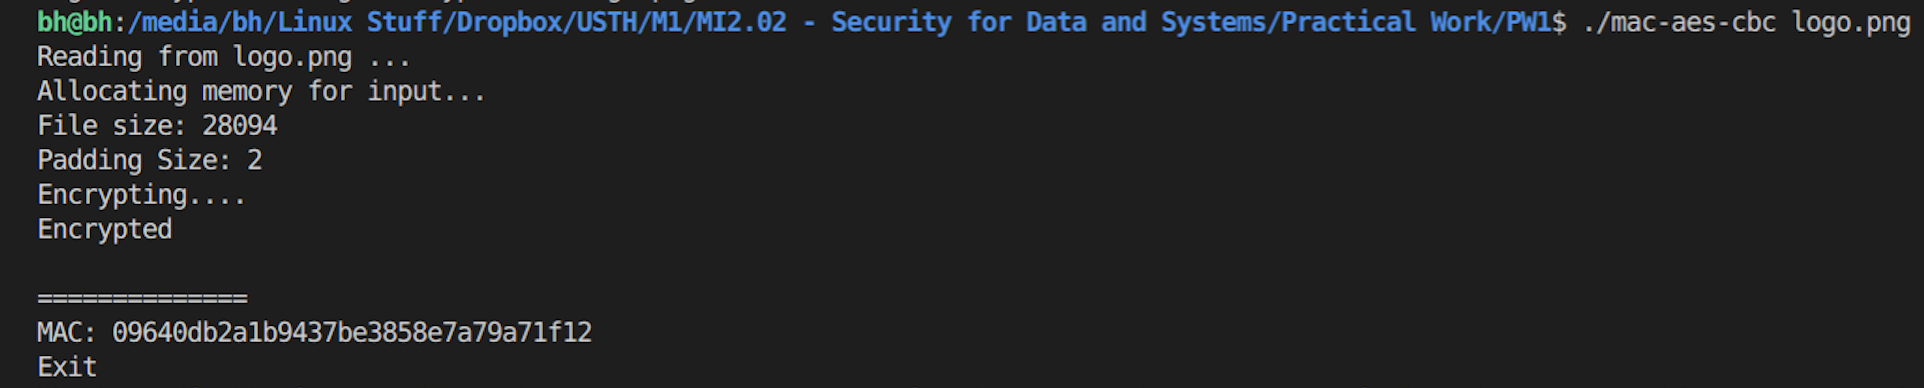
\includegraphics[width=\linewidth]{macoutput}
\\ 


And the task of the last exercise in this practical work is to verifies the consistency between a file and a MAC value given as a string made of only hexadecimal digits in order to check whether the MAC is correctly verified for this file or not. Each iteration compares 1 byte of MAC to 2 characters of argv[2] to find out whether they are consistent with each other. 
\\


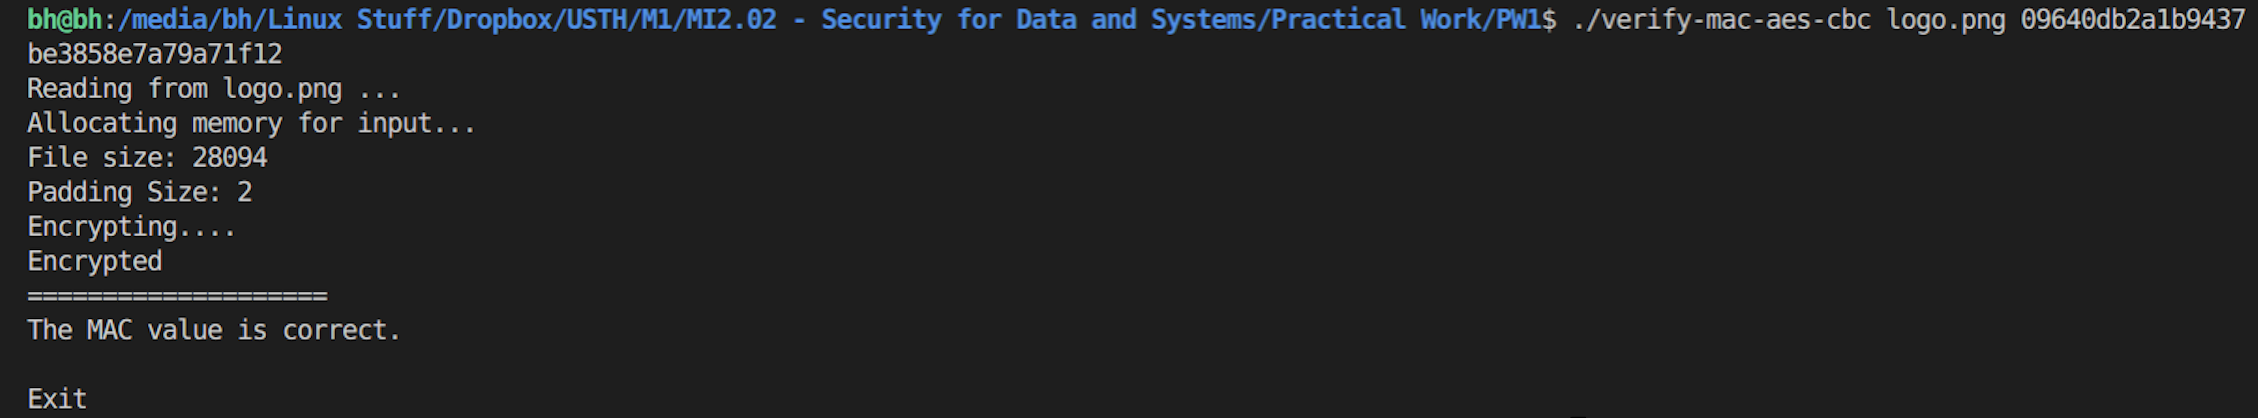
\includegraphics[width=\linewidth]{verify}
\\

\section{The RSA Cryptosystem}
This practical work contains 2 parts, the first one is about RSA Cryptosystem in standard mode, the second one is RSA Cryptosystem in CRT mode. Each part includes 3 exercises with the same tasks but in 2 different modes. 
\\

The first exercise aims at generating the RSA key of size k bits and public exponent e. After specifying k and e as well as the output file, we define generators, mathematical functions and initialize several variables with the help of GMP library. After that we check if e mod \phi(n)\) exists using prime and invertible property. The program computes and displays the generated key on standard output in hexadecimal form on three lines. 
\\

The second exercise's tasks are to encrypt and decrypt a message using the key of the previous exercise. The number of characters of the message is not limited so in the first exercise, we need to generate a key with the large size (large k bits) in order to have the correct result. 
\\

In the second exercise, first we write the encrypt\_rsa that computes the ciphertext from the input message and decrypt\_rsa function that decrypts the ciphertext using GMP library. Then in the main program, we specify the text message, read the generated key file - output file of the previous exercise and assign the values. Finally we encrypt and decrypt the message using 2 functions declared above. 
\\

The last exercise requires to take a input file and an RSA private key as inputs, and computes the signature of the file using the MD5 hash of the file. After specifying the inputs and reading from the key file, we generate the MD5 string of the input file and then sign that string using the key file. 
\\

Doing the same taks, the programs in CRT mode need modifying only some parts from the original ones in standard mode. In both of the mode, we have e and n as the public key, however, while d is the only private key in the standard mode, the other has more: p, q, dp, dq and Ip. Functions that need to be changed are private key generation, decryption and signing. Because both 2 modes have the same public key so the encrytion remains the same. Nevertheless, they have different set of private key so the decryption is different from each other. 

\end{document}